\documentclass[12pt,t]{beamer}
\usepackage{graphicx}
\setbeameroption{hide notes}
\setbeamertemplate{note page}[plain]

% get rid of junk
\usetheme{default}
\beamertemplatenavigationsymbolsempty
\hypersetup{pdfpagemode=UseNone} % don't show bookmarks on initial view

% font
\usepackage{fontspec}
\setsansfont{TeX Gyre Heros}
\setbeamerfont{note page}{family*=pplx,size=\footnotesize} % Palatino for notes
% "TeX Gyre Heros can be used as a replacement for Helvetica"
% In Unix, unzip the following into ~/.fonts
% In Mac, unzip it, double-click the .otf files, and install using "FontBook"
%   http://www.gust.org.pl/projects/e-foundry/tex-gyre/heros/qhv2.004otf.zip

% named colors
\definecolor{offwhite}{RGB}{249,242,215}
% \definecolor{foreground}{RGB}{255,255,255}
\definecolor{foreground}{RGB}{0,0,0}
% \definecolor{background}{RGB}{24,24,24}
\definecolor{background}{RGB}{255,255,255}
\definecolor{title}{RGB}{107,174,214}
\definecolor{gray}{RGB}{100,100,100}
\definecolor{subtitle}{RGB}{102,255,204}
\definecolor{hilight}{RGB}{20,180,204}
\definecolor{vhilight}{RGB}{255,111,207}
\definecolor{lolight}{RGB}{155,155,155}
%\definecolor{green}{RGB}{125,250,125}

% use those colors
\setbeamercolor{titlelike}{fg=title}
\setbeamercolor{subtitle}{fg=title}
\setbeamercolor{institute}{fg=gray}
\setbeamercolor{normal text}{fg=foreground,bg=background}
\setbeamercolor{item}{fg=foreground} % color of bullets
\setbeamercolor{subitem}{fg=gray}
\setbeamercolor{itemize/enumerate subbody}{fg=gray}
\setbeamertemplate{itemize subitem}{{\textendash}}
\setbeamerfont{itemize/enumerate subbody}{size=\footnotesize}
\setbeamerfont{itemize/enumerate subitem}{size=\footnotesize}

% page number
\setbeamertemplate{footline}{%
    \raisebox{5pt}{\makebox[\paperwidth]{\hfill\makebox[20pt]{\color{gray}
          \scriptsize\insertframenumber}}}\hspace*{5pt}}

% add a bit of space at the top of the notes page
\addtobeamertemplate{note page}{\setlength{\parskip}{12pt}}

% a few macros
\newcommand{\bi}{\begin{itemize}}
\newcommand{\ei}{\end{itemize}}
\newcommand{\ig}{\includegraphics}
\newcommand{\subt}[1]{{\footnotesize \color{subtitle} {#1}}}


% title info
\title{Graphs}
\subtitle{Part 1}
% \subtitle{Theory, Representation, and Algorithms}
\author{Gregor Behnke}
\institute{Institute of Artificial Intelligence\\ Ulm University}
\date{\tiny based on Bjarki Ágúst Guðmundsson's and Tómas Ken Magnússon's\\Competitive Programming}
% \date{\href{http://www.biostat.wisc.edu/~kbroman}{\tt \scriptsize biostat.wisc.edu/{\textasciitilde}kbroman}
% \\[-4pt]
% \href{http://github.com/kbroman}{\tt \scriptsize github.com/kbroman}
% }


% Tikz
\usepackage{tikz}
\usetikzlibrary{arrows,shapes}

% Minted
\usepackage{minted}
\usemintedstyle{tango}
\newminted{cpp}{fontsize=\footnotesize}

% Graph styles
\tikzstyle{vertex}=[circle,fill=black!50,minimum size=15pt,inner sep=0pt, font=\small]
\tikzstyle{selected vertex} = [vertex, fill=vhilight]
\tikzstyle{selected2 vertex} = [vertex, fill=hilight!50, text=black]
\tikzstyle{vertex1} = [vertex, fill=red]
\tikzstyle{vertex2} = [vertex, fill=blue]
\tikzstyle{vertex3} = [vertex, fill=green, text=black]
\tikzstyle{vertex4} = [vertex, fill=yellow, text=black]
\tikzstyle{vertex5} = [vertex, fill=pink, text=black]
\tikzstyle{vertex6} = [vertex, fill=purple]
\tikzstyle{edge} = [draw,thick,-]
\tikzstyle{dedge} = [draw,thick,->]
\tikzstyle{weight} = [font=\scriptsize,pos=0.5]
\tikzstyle{selected edge} = [draw,line width=2pt,-,red!50]
\tikzstyle{ignored edge} = [draw,line width=5pt,-,black!20]





\begin{document}

% title slide
{
    \setbeamertemplate{footline}{} % no page number here
    \frame{
        \titlepage
    }
}

\begin{frame}{Today we're going to cover}
    \vspace{10pt}
    \bi
        \item Graph basics
        \item Graph representation (recap)
        \item DFS and BFS
        \item Connected components
        \item DFS tree
        \item Bridges and Articulation
        \item Strongly connected components
        \item Topological sort
        \item Shortest paths in unweighted graphs
        \item Special graphs
            \bi
                \item Trees
                \item Directed acyclic graphs
                \item Bipartite graphs
            \ei
    \ei
\end{frame}


\begin{frame}{What is a graph?}
    \begin{columns}[T]
        \begin{column}{.6\textwidth}
            \bi
                \onslide<2->{
                    \item Vertices $V$ ($|V| = n$)
                        \bi
                            \item Road intersections
                            \item Computers
                            \item Floors in a house
                            \item Objects
                        \ei
                }
                \onslide<3->{
                    \item Edges $E \subseteq V \times V$ ($|E| = m$)
                        \bi
                            \item Roads
                            \item Ethernet cables
                            \item Stairs or elevators
                            \item Relation between objects
                        \ei
                }
            \ei
        \end{column}%
        \hfill%
        \begin{column}{.6\textwidth}
            \begin{figure}
                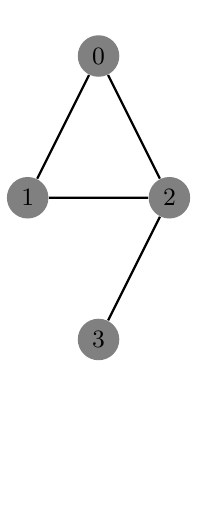
\begin{tikzpicture}[scale=1.8,auto,swap]
                    \onslide<2->{
                        \node[vertex] (0) at (0.5,3) {0};
                        \node[vertex] (1) at (0,2) {1};
                        \node[vertex] (2) at (1,2) {2};
                        \node[vertex] (3) at (0.5,1) {3};
                    }

                    \onslide<3->{
                        \path[edge] (0) -- (1);
                        \path[edge] (0) -- (2);
                        \path[edge] (1) -- (2);
                        \path[edge] (2) -- (3);
                    }
                    \pgfresetboundingbox
                    \path [use as bounding box] (0,0) rectangle (1,3.2);
                \end{tikzpicture}
            \end{figure}
        \end{column}%
    \end{columns}
\end{frame}

\begin{frame}{Types of edges}
    \begin{columns}[T]
        \begin{column}{.6\textwidth}
            \bi
                \item \color<1>{hilight}{Unweighted} \onslide<2->{or \color<2>{hilight} Weighted}
                \onslide<3->{\item \color<3>{hilight} Undirected} \onslide<4->{or \color<4,5>{hilight} Directed}
            \ei
        \end{column}%
        \hfill%
        \begin{column}{.6\textwidth}
            \begin{figure}
                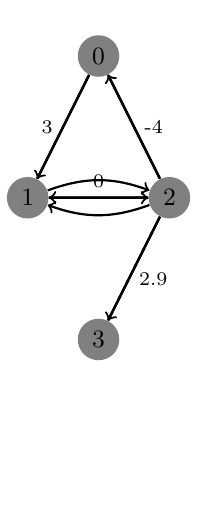
\begin{tikzpicture}[scale=1.8,auto,swap]
                    \node[vertex] (0) at (0.5,3) {0};
                    \node[vertex] (1) at (0,2) {1};
                    \node[vertex] (2) at (1,2) {2};
                    \node[vertex] (3) at (0.5,1) {3};

                    \onslide<1,3>{
                        \path[edge] (0) -- (1);
                        \path[edge] (0) -- (2);
                        \path[edge] (1) -- (2);
                        \path[edge] (2) -- (3);
                    }

                    \onslide<2>{
                        \path[edge] (0) -- node[weight,left] {3} (1);
                        \path[edge] (0) -- node[weight,right] {-4} (2);
                        \path[edge] (1) -- node[weight,above] {0} (2);
                        \path[edge] (2) -- node[weight,right,pos=0.6] {2.9} (3);
                    }

                    \onslide<4-5>{
                        \path[dedge] (0) -- (1);
                        \path[dedge] (2) -- (0);
                        \onslide<4>{
                            \path[dedge] (1) -- (2);
                            \path[dedge] (2) -- (1);
                        }
                        \onslide<5>{
                            \path[dedge] (1) edge[bend left=20] (2);
                            \path[dedge] (2) edge[bend left=20] (1);
                        }
                        \path[dedge] (2) -- (3);
                    }

                    \pgfresetboundingbox
                    \path [use as bounding box] (0,0) rectangle (1,3.2);
                \end{tikzpicture}
            \end{figure}
        \end{column}%
    \end{columns}
\end{frame}


\begin{frame}{Multigraphs}
    \begin{columns}[T]
        \begin{column}{.6\textwidth}
            \bi
                \onslide<2->{\item \color<2>{hilight} Multiple edges}
                \onslide<3->{\item \color<3>{hilight} Self-loops}
            \ei
        \end{column}%
        \hfill%
        \begin{column}{.6\textwidth}
            \begin{figure}
                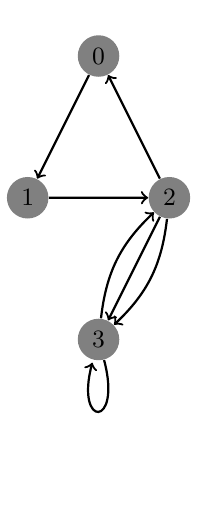
\begin{tikzpicture}[scale=1.8,auto,swap]
                    \node[vertex] (0) at (0.5,3) {0};
                    \node[vertex] (1) at (0,2) {1};
                    \node[vertex] (2) at (1,2) {2};
                    \node[vertex] (3) at (0.5,1) {3};

                    \path[dedge] (0) -- (1);
                    \path[dedge] (2) -- (0);
                    \path[dedge] (2) -- (3);
                    \path[dedge] (1) -- (2);

                    \onslide<2>{
                        \path[dedge] (2) edge[bend left=20] (3);
                        \path[dedge] (3) edge[bend left=20] (2);
                    }

                    \onslide<3>{
                        \path[dedge] (3) edge[loop below] (3);
                    }

                    \pgfresetboundingbox
                    \path [use as bounding box] (0,0) rectangle (1,3.2);
                \end{tikzpicture}
            \end{figure}
        \end{column}%
    \end{columns}
\end{frame}


% TODO: Graph representation (recap)
\begin{frame}[fragile]{Adjacency list}

    \begin{columns}[T]
        \begin{column}{.4\textwidth}
            \begin{minted}{cpp}
0: 1, 2
1: 0, 2
2: 0, 1, 3
3: 2

vi adj[4];
adj[0].push_back(1);
adj[0].push_back(2);
adj[1].push_back(0);
adj[1].push_back(2);
adj[2].push_back(0);
adj[2].push_back(1);
adj[2].push_back(3);
adj[3].push_back(2);
            \end{minted}
        \end{column}%
        \hfill%
        \begin{column}{.4\textwidth}
            \begin{figure}
                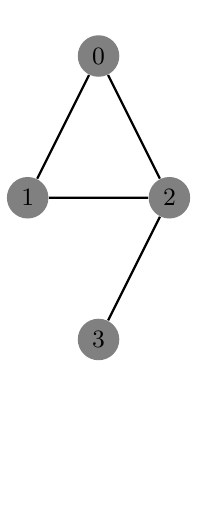
\begin{tikzpicture}[scale=1.8,auto,swap]
                    \node[vertex] (0) at (0.5,3) {0};
                    \node[vertex] (1) at (0,2) {1};
                    \node[vertex] (2) at (1,2) {2};
                    \node[vertex] (3) at (0.5,1) {3};

                    \path[edge] (0) -- (1);
                    \path[edge] (2) -- (0);
                    \path[edge] (2) -- (3);
                    \path[edge] (1) -- (2);

                    \pgfresetboundingbox
                    \path [use as bounding box] (0,0) rectangle (1,3.2);
                \end{tikzpicture}
            \end{figure}
        \end{column}%
    \end{columns}
\end{frame}


\begin{frame}[fragile]{Adjacency list (directed)}

    \begin{columns}[T]
        \begin{column}{.4\textwidth}
            \begin{minted}{cpp}
0: 1
1: 2
2: 0, 1, 3
3:

vi adj[4];
adj[0].push_back(1);
adj[1].push_back(2);
adj[2].push_back(0);
adj[2].push_back(1);
adj[2].push_back(3);
            \end{minted}
        \end{column}%
        \hfill%
        \begin{column}{.4\textwidth}
            \begin{figure}
                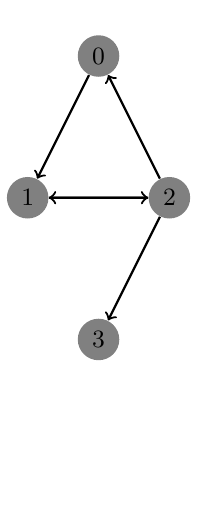
\begin{tikzpicture}[scale=1.8,auto,swap]
                    \node[vertex] (0) at (0.5,3) {0};
                    \node[vertex] (1) at (0,2) {1};
                    \node[vertex] (2) at (1,2) {2};
                    \node[vertex] (3) at (0.5,1) {3};

                    \path[dedge] (0) -- (1);
                    \path[dedge] (2) -- (0);
                    \path[dedge] (2) -- (3);
                    \path[dedge] (1) -- (2);
                    \path[dedge] (2) -- (1);

                    \pgfresetboundingbox
                    \path [use as bounding box] (0,0) rectangle (1,3.2);
                \end{tikzpicture}
            \end{figure}
        \end{column}%
    \end{columns}
\end{frame}



\begin{frame}[fragile]{Vertex properties (undirected graph)}
    \begin{columns}[T]
        \begin{column}{.6\textwidth}
            \vspace{20pt}
            \bi
                \item Degree of a vertex
                    \bi
                        \item Number of adjacent edges
                        \item Number of adjacent vertices
                    \ei
% 
%                 \item In terms of our adjacency list:
%                     \begin{minted}{cpp}
%   adj[v].size()
%                     \end{minted}
%                     \vspace{20pt}

                \onslide<3->{
                    \item Handshaking lemma
                        $$ \sum_{v\in V} \mathrm{deg}(v) = 2m $$
                    \onslide<4->{
                        $$
                            2 + 2 + 3 + 1 = 2\times 4
                        $$
                    }
                }
            \ei
        \end{column}%
        \hfill%
        \begin{column}{.6\textwidth}
            \begin{figure}
                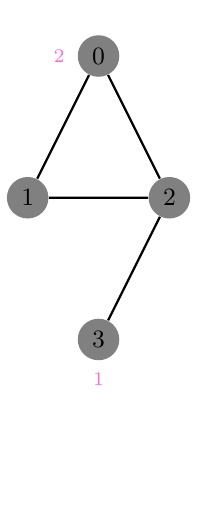
\begin{tikzpicture}[scale=1.8,auto,swap]
                    \node[vertex] (0) at (0.5,3) {0};
                    \node[vertex] (1) at (0,2) {1};
                    \node[vertex] (2) at (1,2) {2};
                    \node[vertex] (3) at (0.5,1) {3};

                    \path[edge] (0) -- (1);
                    \path[edge] (2) -- (0);
                    \path[edge] (2) -- (3);
                    \path[edge] (1) -- (2);

                    \onslide<2->{
                        \node[font=\scriptsize,shift={(-0.5,0)},color=vhilight] at (0) {2};
                        \node[font=\scriptsize,shift={(-0.5,0)},color=vhilight] at (1) {2};
                        \node[font=\scriptsize,shift={(0.5,0)},color=vhilight] at (2) {3};
                        \node[font=\scriptsize,shift={(0,-0.5)},color=vhilight] at (3) {1};
                    }
                    \pgfresetboundingbox
                    \path [use as bounding box] (0,0) rectangle (1,3.2);
                \end{tikzpicture}
            \end{figure}
        \end{column}%
    \end{columns}
\end{frame}



\begin{frame}{Representing graphs}
    \vspace{20pt}
    \bi
        \item There are many types of graphs:
            \bi
                \item Directed vs. undirected
                \item Weighted vs. unweighted
                \item Simple vs. non-simple
            \ei
        \item Many ways to represent graphs
        \item Some special graphs (like trees) have special representations
        \item Most commonly used (general) representations:
            \begin{enumerate}
                \item Adjacency list
                \item Adjacency matrix
                \item Edge list
            \end{enumerate}
    \ei
\end{frame}

% TODO: also show directed and weighted versions
\begin{frame}[fragile]{Adjacency list}

    \begin{columns}[T]
        \begin{column}{.4\textwidth}
            \begin{minted}{cpp}
0: 1, 2
1: 0, 2
2: 0, 1, 3
3: 2

vi adj[4];
adj[0].push_back(1);
adj[0].push_back(2);
adj[1].push_back(0);
adj[1].push_back(2);
adj[2].push_back(0);
adj[2].push_back(1);
adj[2].push_back(2);
adj[3].push_back(2);
            \end{minted}
        \end{column}%
        \hfill%
        \begin{column}{.4\textwidth}
            \begin{figure}
                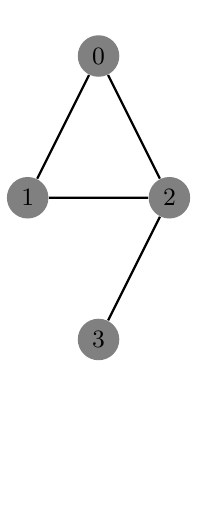
\begin{tikzpicture}[scale=1.8,auto,swap]
                    \node[vertex] (0) at (0.5,3) {0};
                    \node[vertex] (1) at (0,2) {1};
                    \node[vertex] (2) at (1,2) {2};
                    \node[vertex] (3) at (0.5,1) {3};

                    \path[edge] (0) -- (1);
                    \path[edge] (2) -- (0);
                    \path[edge] (2) -- (3);
                    \path[edge] (1) -- (2);

                    \pgfresetboundingbox
                    \path [use as bounding box] (0,0) rectangle (1,3.2);
                \end{tikzpicture}
            \end{figure}
        \end{column}%
    \end{columns}
\end{frame}

\begin{frame}[fragile]{Adjacency matrix}

    \begin{columns}[T]
        \begin{column}{.4\textwidth}
            \begin{minted}{cpp}

0 1 1 0
1 0 1 0
1 1 0 1
0 0 1 0

bool adj[4][4];
adj[0][1] = true;
adj[0][2] = true;
adj[1][0] = true;
adj[1][2] = true;
adj[2][0] = true;
adj[2][1] = true;
adj[2][3] = true;
adj[3][2] = true;
            \end{minted}
        \end{column}%
        \hfill%
        \begin{column}{.4\textwidth}
            \begin{figure}
                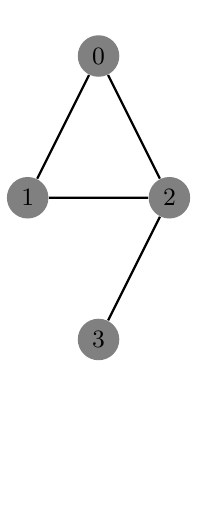
\begin{tikzpicture}[scale=1.8,auto,swap]
                    \node[vertex] (0) at (0.5,3) {0};
                    \node[vertex] (1) at (0,2) {1};
                    \node[vertex] (2) at (1,2) {2};
                    \node[vertex] (3) at (0.5,1) {3};

                    \path[edge] (0) -- (1);
                    \path[edge] (2) -- (0);
                    \path[edge] (2) -- (3);
                    \path[edge] (1) -- (2);

                    \pgfresetboundingbox
                    \path [use as bounding box] (0,0) rectangle (1,3.2);
                \end{tikzpicture}
            \end{figure}
        \end{column}%
    \end{columns}
\end{frame}

\begin{frame}[fragile]{Edge list}

    \begin{columns}[T]
        \begin{column}{.4\textwidth}
            \begin{minted}{cpp}

0, 1
0, 2
1, 2
2, 3



vector<pair<int, int> > edges;
edges.push_back(make_pair(0, 1));
edges.push_back(make_pair(0, 2));
edges.push_back(make_pair(1, 2));
edges.push_back(make_pair(2, 3));
            \end{minted}
        \end{column}%
        \hfill%
        \begin{column}{.4\textwidth}
            \begin{figure}
                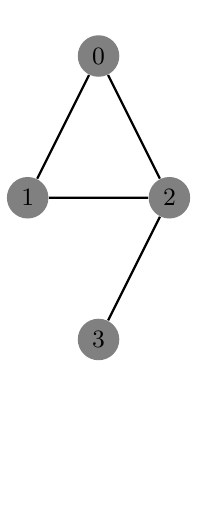
\begin{tikzpicture}[scale=1.8,auto,swap]
                    \node[vertex] (0) at (0.5,3) {0};
                    \node[vertex] (1) at (0,2) {1};
                    \node[vertex] (2) at (1,2) {2};
                    \node[vertex] (3) at (0.5,1) {3};

                    \path[edge] (0) -- (1);
                    \path[edge] (2) -- (0);
                    \path[edge] (2) -- (3);
                    \path[edge] (1) -- (2);

                    \pgfresetboundingbox
                    \path [use as bounding box] (0,0) rectangle (1,3.2);
                \end{tikzpicture}
            \end{figure}
        \end{column}%
    \end{columns}
\end{frame}

\begin{frame}{Efficiency}

    \vspace{20pt}

    {
        \scriptsize
    \begin{center}
        \begin{tabular}{lccc}
            & Adjacency list & Adjacency matrix & Edge list \\
            Storage & $O(|V| + |E|)$ & $O(|V|^2)$ & $O(|E|)$ \\
            Add vertex & $O(1)$ & $O(|V|^2)$ & $O(1)$ \\
            Add edge & $O(1)$ & $O(1)$ & $O(1)$ \\
            Remove vertex & $O(|E|)$ & $O(|V|^2)$ & $O(|E|)$ \\
            Remove edge & $O(|E|)$ & $O(1)$ & $O(|E|)$ \\
            Query: are $u,v$ adjacent? & $O(|V|)$ & $O(1)$ & $O(|E|)$ \\
        \end{tabular}
    \end{center}
    }

    \bi
        \item Different representations are good for different situations
    \ei
\end{frame}


\begin{frame}[fragile]{Vertex properties (undirected graph)}

    \begin{columns}[T]
        \begin{column}{.4\textwidth}
            \begin{minted}{cpp}
0: 1, 2
1: 0, 2
2: 0, 1, 3
3: 2

adj[0].size() // 2
adj[1].size() // 2
adj[2].size() // 3
adj[3].size() // 1
            \end{minted}
        \end{column}%
        \hfill%
        \begin{column}{.4\textwidth}
            \begin{figure}
                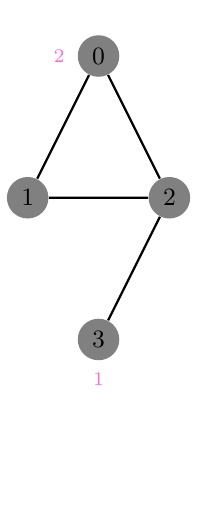
\begin{tikzpicture}[scale=1.8,auto,swap]
                    \node[vertex] (0) at (0.5,3) {0};
                    \node[vertex] (1) at (0,2) {1};
                    \node[vertex] (2) at (1,2) {2};
                    \node[vertex] (3) at (0.5,1) {3};

                    \path[edge] (0) -- (1);
                    \path[edge] (2) -- (0);
                    \path[edge] (2) -- (3);
                    \path[edge] (1) -- (2);

                    \node[font=\scriptsize,shift={(-0.5,0)},color=vhilight] at (0) {2};
                    \node[font=\scriptsize,shift={(-0.5,0)},color=vhilight] at (1) {2};
                    \node[font=\scriptsize,shift={(0.5,0)},color=vhilight] at (2) {3};
                    \node[font=\scriptsize,shift={(0,-0.5)},color=vhilight] at (3) {1};

                    \pgfresetboundingbox
                    \path [use as bounding box] (0,0) rectangle (1,3.2);
                \end{tikzpicture}
            \end{figure}
        \end{column}%
    \end{columns}
\end{frame}


\begin{frame}{Vertex properties (directed graph)}
    \begin{columns}[T]
        \begin{column}{.6\textwidth}
            \bi
                \onslide<1->{
                    \item Outdegree of a vertex $deg^+(v)$
                        \bi
                            \item Number of outgoing edges
                        \ei
                }
                \onslide<3->{
                    \item Indegree of a vertex $deg^-(v)$
                        \bi
                            \item Number of incoming edges
                        \ei
                }
            \ei
        \end{column}%
        \hfill%
        \begin{column}{.6\textwidth}
            \begin{figure}
                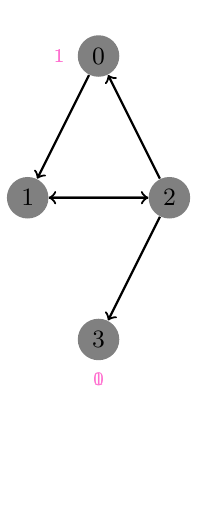
\begin{tikzpicture}[scale=1.8,auto,swap]
                    \node[vertex] (0) at (0.5,3) {0};
                    \node[vertex] (1) at (0,2) {1};
                    \node[vertex] (2) at (1,2) {2};
                    \node[vertex] (3) at (0.5,1) {3};

                    \path[dedge] (0) -- (1);
                    \path[dedge] (2) -- (0);
                    \path[dedge] (2) -- (3);
                    \path[dedge] (1) -- (2);
                    \path[dedge] (2) -- (1);

                    \onslide<2,6>{
                        \node[font=\scriptsize,shift={(-0.5,0)},color=vhilight] at (0) {1};
                        \node[font=\scriptsize,shift={(-0.5,0)},color=vhilight] at (1) {1};
                        \node[font=\scriptsize,shift={(0.5,0)},color=vhilight] at (2) {3};
                        \node[font=\scriptsize,shift={(0,-0.5)},color=vhilight] at (3) {0};
                    }

                    \onslide<4>{
                        \node[font=\scriptsize,shift={(-0.5,0)},color=vhilight] at (0) {1};
                        \node[font=\scriptsize,shift={(-0.5,0)},color=vhilight] at (1) {2};
                        \node[font=\scriptsize,shift={(0.5,0)},color=vhilight] at (2) {1};
                        \node[font=\scriptsize,shift={(0,-0.5)},color=vhilight] at (3) {1};
                    }




                    \pgfresetboundingbox
                    \path [use as bounding box] (0,0) rectangle (1,3.2);
                \end{tikzpicture}
            \end{figure}
        \end{column}%
    \end{columns}
\end{frame}


\begin{frame}[fragile]{Adjacency list (directed)}

    \begin{columns}[T]
        \begin{column}{.4\textwidth}
            \begin{minted}{cpp}
0: 1
1: 2
2: 0, 1, 3
3:

adj[0].size() // 1
adj[1].size() // 1
adj[2].size() // 3
adj[3].size() // 0
            \end{minted}
        \end{column}%
        \hfill%
        \begin{column}{.4\textwidth}
            \begin{figure}
                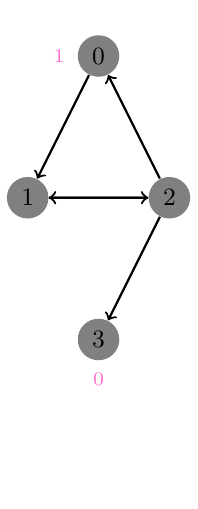
\begin{tikzpicture}[scale=1.8,auto,swap]
                    \node[vertex] (0) at (0.5,3) {0};
                    \node[vertex] (1) at (0,2) {1};
                    \node[vertex] (2) at (1,2) {2};
                    \node[vertex] (3) at (0.5,1) {3};

                    \path[dedge] (0) -- (1);
                    \path[dedge] (2) -- (0);
                    \path[dedge] (2) -- (3);
                    \path[dedge] (1) -- (2);
                    \path[dedge] (2) -- (1);

                    \node[font=\scriptsize,shift={(-0.5,0)},color=vhilight] at (0) {1};
                    \node[font=\scriptsize,shift={(-0.5,0)},color=vhilight] at (1) {1};
                    \node[font=\scriptsize,shift={(0.5,0)},color=vhilight] at (2) {3};
                    \node[font=\scriptsize,shift={(0,-0.5)},color=vhilight] at (3) {0};

                    \pgfresetboundingbox
                    \path [use as bounding box] (0,0) rectangle (1,3.2);
                \end{tikzpicture}
            \end{figure}
        \end{column}%
    \end{columns}
\end{frame}


\begin{frame}{Paths}
    \begin{columns}[T]
        \begin{column}{.6\textwidth}
            \bi
                \item Path / Walk / Trail:
                    $$
                        e_1 e_2 \ldots e_k
                    $$
                such that
                    $$ e_i \in E $$
                    $$ e_i = e_j \Rightarrow i = j $$
                    $$ \mathrm{to}(e_i) = \mathrm{from}(e_{i+1})$$
            \ei
        \end{column}%
        \hfill%
        \begin{column}{.6\textwidth}
            \begin{figure}
                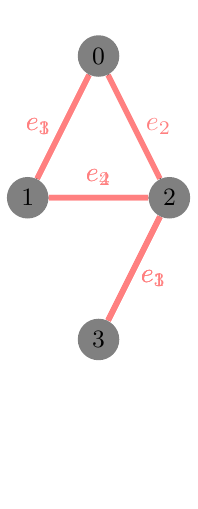
\begin{tikzpicture}[scale=1.8,auto,swap]
                    \node[vertex] (0) at (0.5,3) {0};
                    \node[vertex] (1) at (0,2) {1};
                    \node[vertex] (2) at (1,2) {2};
                    \node[vertex] (3) at (0.5,1) {3};

                    \onslide<1>{
                        \path[edge] (0) -- (1);
                        \path[edge] (2) -- (0);
                        \path[edge] (2) -- (3);
                        \path[edge] (1) -- (2);
                    }

                    \onslide<2>{
                        \path[selected edge] (0) -- node[left] {$e_1$} (1);
                        \path[edge] (2) -- (0);
                        \path[selected edge] (2) -- node[right,pos=0.6] {$e_3$} (3);
                        \path[selected edge] (1) -- node[above] {$e_2$} (2);
                    }

                    \onslide<3>{
                        \path[edge] (0) -- (1);
                        \path[edge] (2) -- (0);
                        \path[selected edge] (2) -- node[right,pos=0.6] {$e_1$} (3);
                        \path[edge] (1) -- (2);
                    }

                    \onslide<4>{
                        \path[selected edge] (0) -- node[left] {$e_3$} (1);
                        \path[selected edge] (2) -- node[right] {$e_2$} (0);
                        \path[selected edge] (2) -- node[right,pos=0.6] {$e_1$} (3);
                        \path[selected edge] (1) -- node[above] {$e_4$} (2);
                    }

                    \pgfresetboundingbox
                    \path [use as bounding box] (0,0) rectangle (1,3.2);
                \end{tikzpicture}
            \end{figure}
        \end{column}%
    \end{columns}
\end{frame}

\begin{frame}{Cycles}
    \begin{columns}[T]
        \begin{column}{.6\textwidth}
            \bi
                \item Cycle / Circuit / Tour:
                    $$
                        e_1 e_2 \ldots e_k
                    $$
                such that
                    $$ e_i \in E $$
                    $$ e_i = e_j \Rightarrow i = j $$
                    $$ \mathrm{to}(e_i) = \mathrm{from}(e_{i+1})$$
                    $$ \color<1>{vhilight}{\mathrm{from}(e_1) = \mathrm{to}(e_{k})} $$
            \ei
        \end{column}%
        \hfill%
        \begin{column}{.6\textwidth}
            \begin{figure}
                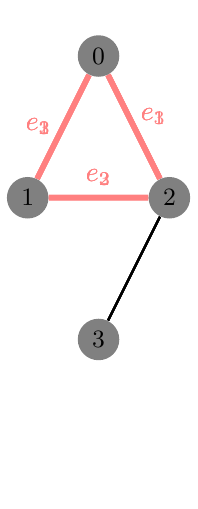
\begin{tikzpicture}[scale=1.8,auto,swap]
                    \node[vertex] (0) at (0.5,3) {0};
                    \node[vertex] (1) at (0,2) {1};
                    \node[vertex] (2) at (1,2) {2};
                    \node[vertex] (3) at (0.5,1) {3};

                    \onslide<1>{
                        \path[edge] (0) -- (1);
                        \path[edge] (2) -- (0);
                        \path[edge] (2) -- (3);
                        \path[edge] (1) -- (2);
                    }

                    \onslide<2>{
                        \path[selected edge] (0) -- node[left] {$e_1$} (1);
                        \path[selected edge] (2) -- node[right,pos=0.6] {$e_3$} (0);
                        \path[edge] (2) -- (3);
                        \path[selected edge] (1) -- node[above] {$e_2$} (2);
                    }

                    \onslide<3>{
                        \path[selected edge] (0) -- node[left] {$e_2$} (1);
                        \path[selected edge] (2) -- node[right,pos=0.6] {$e_1$} (0);
                        \path[edge] (2) -- (3);
                        \path[selected edge] (1) -- node[above] {$e_3$} (2);
                    }

                    \onslide<4>{
                        \path[selected edge] (0) -- node[left] {$e_3$} (1);
                        \path[selected edge] (2) -- node[right,pos=0.6] {$e_1$} (0);
                        \path[edge] (2) -- (3);
                        \path[selected edge] (1) -- node[above] {$e_2$} (2);
                    }

                    \pgfresetboundingbox
                    \path [use as bounding box] (0,0) rectangle (1,3.2);
                \end{tikzpicture}
            \end{figure}
        \end{column}%
    \end{columns}
\end{frame}

% TODO: Graph modeling

% TODO: Depth-first search
\begin{frame}{Depth-first search}
    \vspace{10pt}
    \bi
\item Given a graph (either directed or undirected) and two vertices $u$ and $v$, does there exist a path from $u$ to $v$?
\item Depth-first search is an algorithm for finding such a path, if one exists
    \vspace{10pt}

\item It traverses the graph in depth-first order, starting from the initial vertex $u$
\item We don't actually have to specify a $v$, since we can just let it visit all reachable vertices from $u$ (and still same time complexity)
    \ei
\end{frame}

\begin{frame}[fragile]{Depth-first search}
  \begin{figure}
    \begin{tikzpicture}[auto,swap]
      \node[vertex] (0) at (-0.3,2) {0};
      \node[vertex] (1) at (0.0,-0.5) {1};
      \node[vertex] (2) at (1.9,0.7) {2};
      \node[vertex] (3) at (2.4,2.7) {3};
      \node[vertex] (4) at (3.4,-0.8) {4};
      \node[vertex] (5) at (3.9,1) {5};
      \node[vertex] (6) at (6.2,1.1) {6};
      \node[vertex] (7) at (6.1,-0.9) {7};
      \node[vertex] (8) at (5.7,3.2) {8};
      \node[vertex] (9) at (8.3,2.1) {9};
      \node[vertex] (10) at (8.1,0.1) {10};

      \path[dedge] (0) -- (1);
      \path[dedge] (0) -- (2);

      \path[dedge] (1) -- (4);

      \path[dedge] (2) -- (1);
      \path[dedge] (2) -- (3);

      \path[dedge] (3) -- (0);

      \path[dedge] (4) -- (5);

      \path[dedge] (5) -- (2);
      \path[dedge] (5) -- (3);
      \path[dedge] (5) -- (6);
      \path[dedge] (5) -- (7);
      \path[dedge] (5) -- (8);

      \path[dedge] (6) -- (8);
      \path[dedge] (6) -- (7);

      \path[dedge] (8) to [bend left] (9);

      \path[dedge] (9) to [bend left] (8);

      \path[dedge] (7) -- (10);

      \only<2-4>{\node[vertex,fill=vhilight] (0) at (0) {0};}
      \only<3-4>{
        \path[dedge,vhilight] (0) -- (1);
        \path[dedge,vhilight] (0) -- (2);
      }

      \only<5->{
        \node[vertex,fill=title] (0) at (0) {0};
        \path[dedge,title] (0) -- (1);
        \path[dedge,title] (0) -- (2);
      }

      \only<5-7>{\node[vertex,fill=vhilight] (2) at (2) {2};}
      \only<6-7>{\path[dedge,vhilight] (2) -- (3);}

      \only<8->{
        \node[vertex,fill=title] (2) at (2) {2};
        \path[dedge,title] (2) -- (3);
      }

      \only<8>{\node[vertex,fill=vhilight] (3) at (3) {3};}
      \only<9->{\node[vertex,fill=title] (3) at (3) {3};}

      \only<9-11>{\node[vertex, fill=vhilight] (1) at (1) {1};}
      \only<10-11>{\path[dedge,vhilight] (1) -- (4);}

      \only<12->{
        \node[vertex,fill=title] (1) at (1) {1};
        \path[dedge,title] (1) -- (4);
      }

      \only<12-14>{\node[vertex,fill=vhilight] (4) at (4) {4};}
      \only<13-14>{\path[dedge,vhilight] (4) -- (5);}

      \only<15->{
        \node[vertex,fill=title] (4) at (4) {4};
        \path[dedge,title] (4) -- (5);
      }

      \only<15-17>{\node[vertex,fill=vhilight] (5) at (5) {5};}
      \only<16-17>{
        \path[dedge,vhilight] (5) -- (6);
        \path[dedge,vhilight] (5) -- (7);
        \path[dedge,vhilight] (5) -- (8);
      }

      \only<18->{
        \node[vertex,fill=title] (5) at (5) {5};
        \path[dedge,title] (5) -- (6);
        \path[dedge,title] (5) -- (7);
        \path[dedge,title] (5) -- (8);
      }
      \only<18-20>{\node[vertex,fill=vhilight] (8) at (8) {8};}
      \only<19-20>{\path[dedge,vhilight] (8) to[bend left] (9)};

      \only<21>{\node[vertex,fill=vhilight] (9) at (9) {9};}
      \only<21->{
        \node[vertex,fill=title] (8) at (8) {8};
        \path[dedge,title] (8) to[bend left] (9);
      }
      \only<22->{\node[vertex,fill=title] (9) at (9) {9};}

      \only<22>{\node[vertex,fill=vhilight] (6) at (6) {6};}
      \only<23->{\node[vertex,fill=title] (6) at (6) {6};}

      \only<23-25>{\node[vertex,fill=vhilight] (7) at (7) {7};}
      \only<24-25>{\path[dedge,title] (7) -- (10)};

      \only<26->{\node[vertex,fill=title] (7) at (7) {7};}
      \only<26>{\node[vertex,fill=vhilight] (10) at (10) {10};}
      \only<27->{\node[vertex,fill=title] (10) at (10) {10};}

    \end{tikzpicture}
  \end{figure}

  \texttt{ \begin{tabular}{l c l}
    Stack: &\only<2-4>{{\color{vhilight}0}}\only<5-7>{{\color{vhilight}2}}\only<8>{{\color{vhilight}3}}\only<9-11>{{\color{vhilight}1}}\only<12-14>{{\color{vhilight}4}}\only<15-17>{{\color{vhilight}5}}\only<18-20>{{\color{vhilight}8}}\only<21>{{\color{vhilight}9}}\only<22>{{\color{vhilight}6}}\only<23-25>{{\color{vhilight}7}}\only<26>{{\color{vhilight}10}}  |&\only<4>{2 1}\only<5-6>{1}\only<7>{3 1}\only<8>{1}\only<9-10>{}\only<11>{4}\only<12-13>{}\only<14>{5}\only<15-16>{}\only<17>{8 6 7}\only<18-19>{6 7}\only<20>{9 6 7}\only<21>{6 7}\only<23-24>{}\only<25>{10}\only<26>{}
  \end{tabular}}
  \vspace{10pt}
  \texttt{
    \begin{tabular}{l | c c c c c c c c c c c }
      & 0 & 1 & 2 & 3 & 4 & 5 & 6 & 7 & 8 & 9 & 10 \\
      marked 
      & \only<1>{0}\only<2->{{\color{title}1}} 
      & \only<1-3>{0}\only<4->{{\color{title}1}} 
      & \only<1-3>{0}\only<4->{{\color{title}1}} 
      & \only<1-6>{0}\only<7->{{\color{title}1}} 
      & \only<1-10>{0}\only<11->{{\color{title}1}} 
      & \only<1-13>{0}\only<14->{{\color{title}1}} 
      & \only<1-16>{0}\only<17->{{\color{title}1}} 
      & \only<1-16>{0}\only<17->{{\color{title}1}} 
      & \only<1-16>{0}\only<17->{{\color{title}1}} 
      & \only<1-19>{0}\only<20->{{\color{title}1}}
      & \only<1-24>{0}\only<25->{{\color{title}1}} \\
    \end{tabular}}
\end{frame}

\begin{frame}[fragile]{Depth-first search}
    \begin{minted}{cpp}
vi adj[1000];
bool visited[1000];

void dfs(int u) {
    if (visited[u]) return;

    visited[u] = true;

    FORIT(i,adj[u])
        dfs(*i);
}

FOR(i,0,1000) visited[i] = false;
    \end{minted}
\end{frame}

\begin{frame}{Depth-first search}
    \vspace{10pt}
    \bi
\item But what is the time complexity?
\item Each vertex is visited once, and each edge is traversed once
\item $O(n + m)$
%    \vspace{10pt}
%\item Set of edges visited by DFS form a ``spanning'' tree
    \ei
\end{frame}

% TODO: Breadth-first search
\begin{frame}{Breadth-first search}
    \vspace{30pt}
    \bi
        \item There's another search algorithm called Breadth-first search
        \item Only difference is the order in which it visits the vertices
        \item It goes in order of increasing distance from the source vertex
    \ei
\end{frame}


\begin{frame}{Breadth-first search}
  \begin{figure}
    \begin{tikzpicture}[auto, swap]
      \node[vertex] (0) at (-0.3,2) {0};
      \node[vertex] (1) at (0.0,-0.5) {1};
      \node[vertex] (2) at (1.9,0.7) {2};
      \node[vertex] (3) at (2.4,2.7) {3};
      \node[vertex] (4) at (3.4,-0.8) {4};
      \node[vertex] (5) at (3.9,1) {5};
      \node[vertex] (6) at (6.2,1.1) {6};
      \node[vertex] (7) at (6.1,-0.9) {7};
      \node[vertex] (8) at (5.7,3.2) {8};
      \node[vertex] (9) at (8.3,2.1) {9};
      \node[vertex] (10) at (8.1,0.1) {10};

      \path[dedge] (0) -- (1);
      \path[dedge] (0) -- (2);

      \path[dedge] (1) -- (4);

      \path[dedge] (2) -- (1);
      \path[dedge] (2) -- (3);

      \path[dedge] (3) -- (0);

      \path[dedge] (4) -- (5);

      \path[dedge] (5) -- (2);
      \path[dedge] (5) -- (3);
      \path[dedge] (5) -- (6);
      \path[dedge] (5) -- (7);
      \path[dedge] (5) -- (8);

      %\path[dedge] (6) -- (5);
      \path[dedge] (6) -- (8);
      \path[dedge] (6) -- (7);

      %\path[dedge] (8) -- (5);
      \path[dedge] (8) to [bend left] (9);

      \path[dedge] (9) to [bend left] (8);

      \path[dedge] (7) -- (10);

      \only<2-4>{\node[vertex,fill=vhilight] (0) at (-0.3,2) {0};}
      \only<3-4>{
        \path[dedge,vhilight] (0) -- (1);
        \path[dedge,vhilight] (0) -- (2);
      }

      \only<5->{\node[vertex,fill=title] (0) at (0) {0};}
      \only<5->{\path[dedge,thick,title] (0) -- (1);}
      \only<5->{\path[dedge,thick,title] (0) -- (2);}
      \only<5->{\node[vertex,fill=vhilight] (1) at (1) {1};}

      \only<6-7>{\path[dedge,vhilight] (1) -- (4);}
      \only<8->{\path[dedge,thick,title] (1) -- (4);}

      \only<8->{\node[vertex,fill=title] (1) at (1) {1};}
      \only<8-10>{\node[vertex,fill=vhilight] (2) at (2) {2};}
      \only<9-10>{\path[dedge,vhilight] (2) -- (3);}
      \only<8-10>{\node[vertex,fill=vhilight] (2) at (2) {2};}


      \only<10>{\path[dedge,vhilight] (2) -- (3);}
      \only<11->{\node[vertex,fill=title] (2) at (2) {2};}
      \only<11->{\path[dedge,title,thick] (2) -- (3);}
      \only<11-13>{\node[vertex,fill=vhilight] (4) at (4) {4};}
      \only<12-13>{\path[dedge,vhilight] (4) -- (5);}

      \only<14->{\node[vertex,fill=title] (4) at (4) {4};}
      \only<14->{\path[dedge,thick,title] (4) -- (5);}
      \only<14>{\node[vertex,fill=vhilight] (3) at (3) {3};}

      \only<14>{\node[vertex,fill=vhilight] (3) at (3) {3};}
      \only<15->{\node[vertex,fill=title] (3) at (3) {3};}

      \only<15-17>{\node[vertex,fill=vhilight] (5) at (5) {5};}
      \only<16-17>{
        \path[dedge,vhilight] (5) -- (6);
        \path[dedge,vhilight] (5) -- (7);
        \path[dedge,vhilight] (5) -- (8);
      }
      \only<18->{
        \node[vertex,fill=title] (5) at (5) {5};
        \path[dedge,title,thick] (5) -- (6);
        \path[dedge,title,thick] (5) -- (7);
        \path[dedge,title,thick] (5) -- (8);
      }
      \only<18>{ \node[vertex,fill=vhilight] (6) at (6) {6}; }
      \only<19->{ \node[vertex,fill=title] (6) at (6) {6}; }

      \only<19-21>{ \node[vertex,fill=vhilight] (7) at (7) {7}; }
      \only<20-21>{\path[dedge,vhilight] (7) -- (10);}

      \only<22->{ 
        \node[vertex,fill=title] (7) at (7) {7};
        \path[dedge,title,thick] (7) -- (10);
      }

      \only<22-24>{\node[vertex,fill=vhilight] (8) at (8) {8};}
      \only<23-24>{\path[dedge,vhilight] (8) to[bend left] (9)};

      \only<25->{
        \node[vertex,fill=title] (8) at (8) {8};
        \path[dedge,title] (8) to[bend left] (9);
      }
      \only<25>{\node[vertex,fill=vhilight] (10) at (10) {10};}
      \only<26->{\node[vertex,fill=title] (10) at (10) {10};}
      \only<26>{\node[vertex,fill=vhilight] (9) at (9) {9};}
      \only<27->{\node[vertex,fill=title] (9) at (9) {9};}

    \end{tikzpicture}
  \end{figure}

  %\mintinline{cpp}{Queue: }
  \texttt{ \begin{tabular}{l l}
  \texttt{Queue: } & 
   \only<2-3>{{\color{vhilight}0}}\only<4>{{\color{vhilight}0} 1 2}\only<5-6>{{\color{vhilight}1} 2}\only<7>{{\color{vhilight}1} 2 4}\only<8-9>{{\color{vhilight}2} 4}\only<10>{{\color{vhilight}2} 4 3}\only<11-12>{{\color{vhilight}4} 3}\only<13>{{\color{vhilight}4} 3 5}\only<14>{{\color{vhilight}3} 5}\only<15-16>{{\color{vhilight}5}}\only<17>{{\color{vhilight}5} 6 7 8}\only<18>{{\color{vhilight}6} 7 8}\only<19-20>{{\color{vhilight}7} 8}\only<21>{{\color{vhilight}7} 8 10}\only<22-23>{{\color{vhilight}8} 10}\only<24>{{\color{vhilight}8} 10 9}\only<25>{{\color{vhilight}10} 9}\only<26>{{\color{vhilight}9}}
  \end{tabular}}

  \vspace{10pt}
  \texttt{
    \begin{tabular}{l | c c c c c c c c c c c }
      & 0 & 1 & 2 & 3 & 4 & 5 & 6 & 7 & 8 & 9 & 10 \\
      marked 
      & \only<1>{0}\only<2->{{\color{title}1}} 
      & \only<1-3>{0}\only<4->{{\color{title}1}} 
      & \only<1-3>{0}\only<4->{{\color{title}1}} 
      & \only<1-9>{0}\only<10->{{\color{title}1}} 
      & \only<1-6>{0}\only<7->{{\color{title}1}} 
      & \only<1-12>{0}\only<13->{{\color{title}1}} 
      & \only<1-16>{0}\only<17->{{\color{title}1}} 
      & \only<1-16>{0}\only<17->{{\color{title}1}} 
      & \only<1-16>{0}\only<17->{{\color{title}1}} 
      & \only<1-23>{0}\only<24->{{\color{title}1}}
      & \only<1-20>{0}\only<21->{{\color{title}1}} \\
    \end{tabular}}
\end{frame}

\begin{frame}[fragile]{Breadth-first search}
    \begin{minted}[fontsize=\footnotesize]{cpp}
vi adj[1000];
bool visited[1000];

queue<int> Q;
Q.push(start);
visited[start] = true;

while (!Q.empty()) {
    int u = Q.front(); Q.pop();

    FORIT(i,adj[u]) if (!visited[*i]) {
        Q.push(*i);
        visited[*i] = true;
    }
}
    \end{minted}
\end{frame}

% TODO: Shortest path in unweighted graphs
\begin{frame}{Shortest path in unweighted graphs}
    \vspace{5pt}
    \bi
        \item We have an unweighted graph, and want to find the shortest path from $A$ to $B$
        \item That is, we want to find a path from $A$ to $B$ with the minimum number of edges
        \vspace{10pt}
        \item Breadth-first search goes through the vertices in increasing order of distance from the start vertex
        \item Just do a single breadth-first search from $A$, until we find $B$
        \vspace{5pt}
        \item Or let the search continue through the whole graph, and then we have the shortest paths from $A$ to all other vertices
        \item Shortest path from $A$ to all other vertices: $O(n + m)$
    \ei
\end{frame}

\begin{frame}[fragile]{Shortest path in unweighted graphs}

    \begin{minted}[fontsize=\scriptsize]{cpp}
vi adj[1000];
int dist[1000];

FOR(i,0,1000) dist[i] = -1;

queue<int> Q;
Q.push(A);
dist[A] = 0;

while (!Q.empty()) {
    int u = Q.front(); Q.pop();

    FORIT(i,adj[u]) if (dist[*i] == -1) {
        Q.push(*i);
        dist[*i] = 1 + dist[u];
    }
}
    \end{minted}

\end{frame}


% TODO: Flood fill

% TODO: Connected components
\begin{frame}{Connected components}
    \vspace{30pt}
    \bi
        \item An undirected graph can be partitioned into connected components
        \item A connected component is a maximal subset of the vertices such that each pair of vertices is reachable from each other

        \vspace{10pt}

        \item We've already seen this in a couple of problems, but we've been using Union-Find to keep track of the components
    \ei
\end{frame}

\begin{frame}{Connected components}
    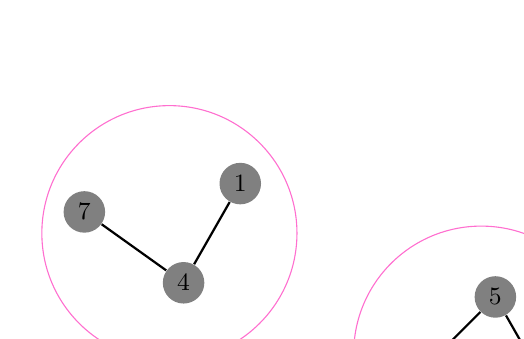
\begin{tikzpicture}[scale=1.8,auto,swap]

        \node[vertex] (1) at (-0.8,1.9) {1};
        \node[vertex] (2) at (3,1.7) {2};
        \node[vertex] (3) at (0.4,0.5) {3};
        \node[vertex] (4) at (-1.2,1.2) {4};
        \node[vertex] (5) at (1,1.1) {5};
        \node[vertex] (6) at (1.4,0.4) {6};
        \node[vertex] (7) at (-1.9,1.7) {7};

        \path[edge] (1) -- (4);
        \path[edge] (4) -- (7);
        \path[edge] (3) -- (5);
        \path[edge] (5) -- (6);
        \path[edge] (6) -- (3);

        \onslide<2->{
            \draw[color=vhilight] (-1.3,1.55) ellipse (0.9cm and 0.9cm);
            \draw[color=vhilight] (0.9,0.7) ellipse (0.9cm and 0.9cm);
            \draw[color=vhilight] (3,1.7) ellipse (0.3cm and 0.3cm);
        }

        \pgfresetboundingbox
        \path [use as bounding box] (-2.3,1.0) rectangle (1,3.0);
    \end{tikzpicture}
\end{frame}

\begin{frame}{Connected components}
    \vspace{30pt}
    \bi
        \item Also possible to find these components using depth-first search
        \item Pick some vertex we don't know anything about, and do a depth-first search out from it
        \item All vertices reachable from that starting vertex are in the same component
        \item Repeat this process until you have all the components
        \item Time complexity is $O(n + m)$
    \ei
\end{frame}

\begin{frame}[fragile]{Connected components}
    \begin{minted}[fontsize=\scriptsize]{cpp}
vi adj[1000];
vi component[1000];

void find_component(int cur_comp, int u) {
    if (component[u] != -1) return;

    component[u] = cur_comp;

    FORIT(i,adj[u]) find_component(cur_comp, *i);
}

int components = 0;
FOR(i,0,n) component[i] = -1;
FOR(u,0,n) if (component[u] == -1) {
    find_component(components, u);
    components++;
}
    \end{minted}
\end{frame}

% TODO: DFS tree
\begin{frame}{Depth-first search tree}
    \vspace{30pt}

    \bi
        \item When we do a depth-first search from a certain vertex, the path
            that we take forms a tree
        \item When we go from a vertex to another vertex that we haven't visited before, the edge that we take is called a \textit{forward edge}
        \item When we go from a vertex to another vertex that we've already visited before, the edge that we take is called a \textit{backward edge}
        \item To be more specific: the forward edges form a ``spanning'' tree
%         \vspace{20pt}
%         \item \textit{see example}
    \ei
\end{frame}

\begin{frame}{Depth-first search tree}
    \vspace{30pt}

    \bi
        \item This tree of forward edges, along with the backward edges, can be analyzed to get a lot of information about the original graph
        \vspace{10pt}
        \item For example: a backward edge represents a cycle in the original graph
        \item If there are no backward edges, then there are no cycles in the original graph (i.e.\ the graph is acyclic)
    \ei
\end{frame}

\begin{frame}{Analysing the DFS tree}
    \vspace{20pt}
    \bi
        \item Let's take a closer look at the depth-first search tree
        \vspace{10pt}
        \item First, let's number each of the vertices in the order that we visit them in the depth-first search
        \item For each vertex, we want to know the smallest number of a vertex that we visited when exploring the subtree rooted at the current vertex ($\rightarrow$ Low-Link number)
        \vspace{10pt}
        \item Why? We'll see in a bit..
%         \vspace{10pt}
%         \item \textit{see example}
    \ei
\end{frame}

\begin{frame}[fragile]{Analysing the DFS tree}
    \begin{minted}[fontsize=\scriptsize]{cpp}
const int n = 1000;
vi adj[n];
int low[n]; int num[n];

int curnum = 0;

void analyze(int u, int p) {
    low[u] = num[u] = curnum++;
    FORIT(i,adj[u]) {
        if (*i == p) continue;
        if (num[*i] == -1) {
            analyze(*i, u);
            low[u] = min(low[u], low[*i]);
        } else low[u] = min(low[u], num[*i]);
    }
}

FOR(i,0,n) num[i] = -1;
FOR(i,0,n) if (num[i] == -1)
    analyze(i, -1);
    \end{minted}
\end{frame}

\begin{frame}{Analysing the DFS tree}
    \vspace{30pt}
    \bi
        \item Time complexity of this is just $O(n + m)$, since this is basically just one depth-first search
        \vspace{20pt}
        \item Now, as promised, let's see some applications of this
    \ei
\end{frame}

% TODO: Articulation points/bridges
\begin{frame}{Bridges and Articulation points}
    \vspace{20pt}
    \bi
        \item We have an undirected graph
        \item Without loss of generality, assume it is connected (i.e.\ one big connected component)
        \item Find an edge -- a bridge, so that if you remove that edge the graph is no longer connected
        \item Find a vertex -- an articulation point, so that if you remove that vertex the graph is no longer connected
        \pause
        \vspace{10pt}
        \item Naive algorithm: Try removing edges, one at a time, and finding the connected components of the resulting graph \pause
        \item That's pretty inefficient, $O(m(n + m))$
    \ei
\end{frame}

\begin{frame}{Bridges and Articulation points}
    \vspace{20pt}
    \bi
        \item Let's take a look at the values that we computed in the DFS tree
        \vspace{10pt} \pause
        \item We see that a forward edge $(u,v)$ is a bridge if and only if \texttt{low[v]} $>$ \texttt{num[u]}
        \vspace{10pt}
        \item Similarly a vertex is an articulation point if it has a successor $u$ with \texttt{low[v]} $\geq$ \texttt{num[u]} (special treatment for the root vertex)
        \vspace{10pt}
        \item Simple to extend our analysis function to return all bridges
        \item Again, this is just $O(n + m)$
    \ei
\end{frame}

\begin{frame}[fragile]{Bridges}
    \begin{minted}[fontsize=\tiny]{cpp}
const int n = 1000;
vi adj[n];
int low[n]; int num[n];
int curnum = 0;

vector<pii> bridges;

void find_bridges(int u, int p) {
    low[u] = num[u] = curnum++;
    FORIT(i,adj[u]) {
        if (*i == p) continue;
        if (num[*i] == -1) {
            find_bridges(*i, u);
            low[u] = min(low[u], low[*i]);
        } else low[u] = min(low[u], num[*i]);

        if (low[*i] > num[u])
            bridges.push_back(make_pair(u, *i));
    }
}

FOR(i,0,n) num[i] = -1;
FOR(i,0,n) if (num[i] == -1) 
    find_bridges(i, -1);
    \end{minted}
\end{frame}

\begin{frame}[fragile]{Articulation points}
    \begin{minted}[fontsize=\tiny]{cpp}
const int n = 1000;
vi adj[n];
int low[n]; int num[n];
int curnum = 0;

vi arti;

void find_arti(int u, int p) {
    low[u] = num[u] = curnum++;
    int nc = 0;
    bool isArti = false;
    FORIT(i,adj[u]) {
        if (*i == p) continue;
        if (num[*i] == -1) {
            nc++;
            find_arti(*i, u);
            low[u] = min(low[u], low[*i]);
            if (low[*i] > num[u]) isArti = true;
        } else low[u] = min(low[u], num[*i]);
    }
    
    if (isArti || (!curnum && nc >= 2))
        arti.push_back(u);
}

FOR(i,0,n) num[i] = -1;
FOR(i,0,n) if (num[i] == -1) 
    find_arti(i, -1);
    \end{minted}
\end{frame}


\begin{frame}{Blockgraphs and Cacti}
  \begin{figure}
    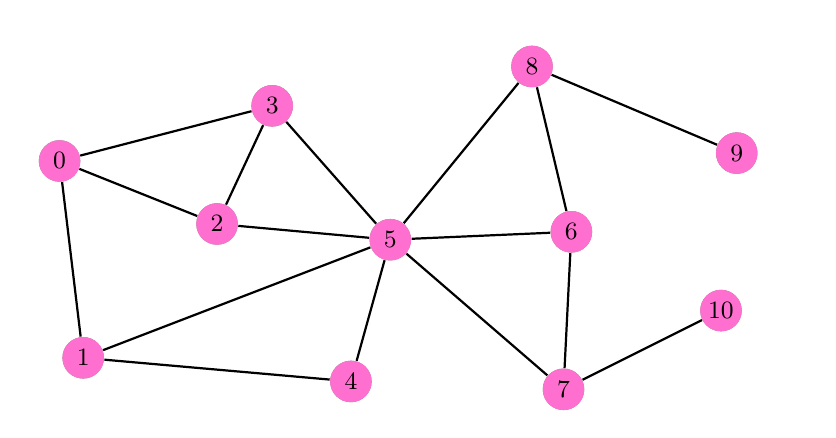
\begin{tikzpicture}[auto, swap]
			\node at (-0.5,3.5) {\phantom{a}};
			\node at (9,3.5) {\phantom{a}};
      \node<1,3->[vertex] (0) at (-0.3,2) {0};
      \node<1,3->[vertex] (1) at (0.0,-0.5) {1};
      \node<1,3->[vertex] (2) at (1.7,1.2) {2};
      \node<1,3->[vertex] (3) at (2.4,2.7) {3};
      \node<1,3->[vertex] (4) at (3.4,-0.8) {4};
	  \node<1,4->[vertex] (5) at (3.9,1) {5};
      \node<2>[selected vertex] (0) at (-0.3,2) {0};
      \node<2>[selected vertex] (1) at (0.0,-0.5) {1};
      \node<2>[selected vertex] (2) at (1.7,1.2) {2};
      \node<2>[selected vertex] (3) at (2.4,2.7) {3};
      \node<2>[selected vertex] (4) at (3.4,-0.8) {4};
	  \node<2-3>[selected vertex] (5) at (3.9,1) {5};
      
			
			
	  \node<1-2,4->[vertex] (6) at (6.2,1.1) {6};
      \node<1-2,5->[vertex] (7) at (6.1,-0.9) {7};
	  \node<1-2,4>[vertex] (8) at (5.7,3.2) {8};
 	  \node<3>[selected vertex] (6) at (6.2,1.1) {6};
      \node<3-4>[selected vertex] (7) at (6.1,-0.9) {7};
	  \node<3,5>[selected vertex] (8) at (5.7,3.2) {8};

			
	  \node<1-4>[vertex] (9) at (8.3,2.1) {9};
      \node<1-3,5>[vertex] (10) at (8.1,0.1) {10};

	  \node<5>[selected vertex] (9) at (8.3,2.1) {9};
      \node<4>[selected vertex] (10) at (8.1,0.1) {10};

      \path[edge] (0) -- (2);

      \path[edge] (1) -- (0);
      \path[edge] (1) -- (4);

      \path[edge] (2) -- (3);

      \path[edge] (3) -- (0);

      \path[edge] (4) -- (5);

      \path[edge] (5) -- (1);
      \path[edge] (5) -- (2);
      \path[edge] (5) -- (3);
      \path[edge] (5) -- (6);
      \path[edge] (5) -- (7);
      \path[edge] (5) -- (8);

      %\path[dedge] (6) -- (5);
      \path[edge] (6) -- (8);
      \path[edge] (6) -- (7);

      %\path[dedge] (8) -- (5);
      \path[edge] (8) to (9);


      \path[edge] (7) -- (10);

       \end{tikzpicture}
  \end{figure}
 	\bi
		\item Every graph can be viewed as a tree of 2-connected components, called \emph{Blocks}
		\item A graph where every block is a clique is called a Blockgraph
		\item A graph where every block is a circle is called a Cactusgraph
	\ei
\end{frame}

% TODO: Strongly connected components
\begin{frame}{Strongly connected components}
    \vspace{10pt}
    \bi
        \item We know how to find connected components in undirected graphs
        \item But what about directed graphs?
        \vspace{10pt}
        \item Such components behave a bit differently in directed graphs, especially since if $v$ is reachable from $u$, it doesn't mean that $u$ is reachable from $v$
        \vspace{10pt}
        \item The definition remains the same, though
        \item A strongly connected component is a maximal subset of the vertices such that each pair of vertices is reachable from each other
    \ei
\end{frame}

\begin{frame}{Strongly connected components}
    \vspace{40pt}
    \bi
        \item The connected components algorithm won't work here
        \vspace{10pt}
        \item Instead we can use the depth-first search tree of the graph to find these components
       % \vspace{10pt}
       % \item \textit{see example}
    \ei
\end{frame}

\begin{frame}[fragile]{Strongly connected components}
\scriptsize
    \begin{minted}[fontsize=\scriptsize]{cpp}
vi adj[1000]; int low[1000]; int num[1000]; int comp[1000];
int ccomp = curnum = 0; stack<int> st;

void scc(int u) {
    st.push(u); low[u] = num[u] = curnum++;
    FORIT(i,adj[u])
        if (num[*i] == -1) {
            scc(*i); low[u] = min(low[u], low[*i]);
        } else if (comp[*i] == -1)
            low[u] = min(low[u], num[*i]);

    if (num[u] == low[u]) {
        while (true) {
            int cur = st.top(); st.pop();
            comp[cur] = ccomp;
            if (cur == u) break;
        }
        ccomp++;
    }
}

FOR(i,0,1000) comp[i] = num[i] = -1;
FOR(i,0,n) if (num[i] == -1)
    scc(i);
    \end{minted}
\end{frame}

\begin{frame}{Strongly connected components}
    \vspace{30pt}
    \bi
        \item Time complexity?
        \item Basically just the DFS analyze function (which was $O(n + m)$), with one additional loop to construct the component
        \item But each vertex is only in one component...
        \item Time complexity still just $O(n + m)$
    \ei
\end{frame}

\begin{frame}{Condensations}
  \begin{figure}
    \begin{tikzpicture}[auto, swap]
			\node at (-0.5,3.5) {\phantom{a}};
			\node at (9,3.5) {\phantom{a}};
      \node<1-2>[vertex] (0) at (-0.3,2) {0};
      \node<1-3>[vertex] (1) at (0.0,-0.5) {1};
			\node[vertex] (2) at (1.7,1.2) {\only<1-2>{2}\only<3->{0,2,3}};
      \node<1-2>[vertex] (3) at (2.4,2.7) {3};
      \node<1-3>[vertex] (4) at (3.4,-0.8) {4};
			\node[vertex] (5) at (3.9,1) {\only<1-3>{5}\only<4->{1,4,5}};
      \node[vertex] (6) at (6.2,1.1) {6};
      \node[vertex] (7) at (6.1,-0.9) {7};
			\node[vertex] (8) at (5.7,3.2) {\only<1>{8}\only<2->{8,9}};
      \node<1>[vertex] (9) at (8.3,2.1) {9};
      \node[vertex] (10) at (8.1,0.1) {10};

      \path<1-2>[dedge] (0) -- (2);

      \path<1-2>[dedge] (1) -- (0);
      \path<3>[dedge] (1) -- (2);
      \path<1-3>[dedge] (1) -- (4);

      \path<1-2>[dedge] (2) -- (3);

      \path<1-2>[dedge] (3) -- (0);

      \path<1-3>[dedge] (4) -- (5);

      \path<1-3>[dedge] (5) -- (1);
      \path[dedge] (5) -- (2);
      \path<1-2>[dedge] (5) -- (3);
      \path[dedge] (5) -- (6);
      \path[dedge] (5) -- (7);
      \path[dedge] (5) -- (8);

      %\path[dedge] (6) -- (5);
      \path[dedge] (6) -- (8);
      \path[dedge] (6) -- (7);

      %\path[dedge] (8) -- (5);
      \path<1>[dedge] (8) to [bend left] (9);

      \path<1>[dedge] (9) to [bend left] (8);

      \path[dedge] (7) -- (10);

       \end{tikzpicture}
  \end{figure}
 \bi
  \item[$\rightarrow$] Once we know all the SCCs we can create an \textbf{abstraction} of the current graph, called its condensation
  \item Replace all SCCs by a single new node
 \ei
\end{frame}

% \begin{frame}{Example problem: Come and Go}
%     \bi
%         \item http://uva.onlinejudge.org/external/118/11838.html
%     \ei
% \end{frame}

% TODO: Topological sort
\begin{frame}{Topological sort}
    \vspace{5pt}
    \bi
        \item We have $n$ tasks
        \item Each task $i$ has a list of tasks that must be finished before we can start task $i$
        \item Find an order in which we can process the tasks
        \vspace{5pt}
        \item Can be represented as a directed graph
            \bi
                \item Each task is a vertex in the graph
                \item If task $j$ should be finished before task $i$, then we add a directed edge from vertex $i$ to vertex $j$
            \ei
        \vspace{5pt}
        \item Notice that this can't be solved if the graph contains a cycle (i.e. is not a DAG)
        \vspace{5pt}
        \item A modified depth-first search can be used to find an ordering in $O(n + m)$ time, or determine that one does not exist
    \ei
\end{frame}

\begin{frame}[fragile]{Topological sort}
    \begin{minted}[fontsize=\scriptsize]{cpp}
vi adj[1000];
bool visited[1000];
vector<int> order;

void topsort(int u) {
    if (visited[u]) return;

    visited[u] = true;
    FORIT(i,adj[u]) topsort(*i);

    order.push_back(u);
}

FOR(i,0,n) visited[i] = false;
FOR(i,0,n) topsort(i);
    \end{minted}
\end{frame}

% \begin{frame}{Example problem: Ordering Tasks}
%     \bi
%         \item http://uva.onlinejudge.org/external/103/10305.html
%     \ei
% \end{frame}


% TODO: Example problem
% TODO: Some common graph problems
\begin{frame}{Known graph problems}
    \vspace{30pt}
    \bi
        \item The problems we're dealing with very often ask us to solve some well known graph problem
        \item But usually it's well hidden in the problem statement
        \vspace{10pt}
        \item Let's take a look at a few examples
    \ei
\end{frame}

% TODO: Minimum vertex cover
\begin{frame}{Maximum clique}
    \bi
        \item We have an unweighted undirected graph
        \item A clique is a subset of the vertices $S$, such that for all $u,v \in S$ with $u \neq v$, there is an edge $(u,v)$
    \ei

    \begin{figure}
        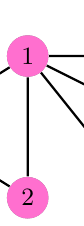
\begin{tikzpicture}[scale=1.8,auto,swap]
            \onslide<1>{
                \node[vertex] (0) at (0,0.5) {0};
                \node[vertex] (1) at (0.8,1) {1};
                \node[vertex] (2) at (0.8,0) {2};
                \node[vertex] (3) at (2,1) {3};
                \node[vertex] (4) at (1.8,0.5) {4};
                \node[vertex] (5) at (1.6,0) {5};
            }
            \onslide<2-4>{
                \node[selected vertex] (0) at (0,0.5) {0};
                \node[selected vertex] (1) at (0.8,1) {1};
                \node[selected vertex] (2) at (0.8,0) {2};
                \node[vertex] (3) at (2,1) {3};
                \node[vertex] (4) at (1.8,0.5) {4};
                \node[vertex] (5) at (1.6,0) {5};
            }

            \path[edge] (0) -- (1);
            \path[edge] (0) -- (2);
            \path[edge] (1) -- (2);
            \path[edge] (1) -- (3);
            \path[edge] (1) -- (4);
            \path[edge] (1) -- (5);

            \pgfresetboundingbox
            \path [use as bounding box] (0.8,0) rectangle (1,1.2);
        \end{tikzpicture}
    \end{figure}

    \vspace{10pt}
    \bi
        \item<3-> We want to find a clique of maximum size
        \vspace{10pt}
        \item<4-> NP-hard problem in general graphs
    \ei
\end{frame}


% TODO: Minimum vertex cover
\begin{frame}{Minimum vertex cover}
    \bi
        \item We have an unweighted undirected graph
        \item A vertex cover is a subset of the vertices $S$, such that for each edge $(u, v)$ in the graph, either $u$ or $v$ (or both) are in $S$
    \ei

    \begin{figure}
        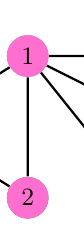
\begin{tikzpicture}[scale=1.8,auto,swap]
            \onslide<1>{
                \node[vertex] (0) at (0,0.5) {0};
                \node[vertex] (1) at (0.8,1) {1};
                \node[vertex] (2) at (0.8,0) {2};
                \node[vertex] (3) at (2,1) {3};
                \node[vertex] (4) at (1.8,0.5) {4};
                \node[vertex] (5) at (1.6,0) {5};
            }
            \onslide<2-3>{
                \node[selected vertex] (0) at (0,0.5) {0};
                \node[selected vertex] (1) at (0.8,1) {1};
                \node[vertex] (2) at (0.8,0) {2};
                \node[vertex] (3) at (2,1) {3};
                \node[selected vertex] (4) at (1.8,0.5) {4};
                \node[vertex] (5) at (1.6,0) {5};
            }
            \onslide<4->{
                \node[vertex] (0) at (0,0.5) {0};
                \node[selected vertex] (1) at (0.8,1) {1};
                \node[selected vertex] (2) at (0.8,0) {2};
                \node[vertex] (3) at (2,1) {3};
                \node[vertex] (4) at (1.8,0.5) {4};
                \node[vertex] (5) at (1.6,0) {5};
            }

            \path[edge] (0) -- (1);
            \path[edge] (0) -- (2);
            \path[edge] (1) -- (2);
            \path[edge] (1) -- (3);
            \path[edge] (1) -- (4);
            \path[edge] (1) -- (5);

            \pgfresetboundingbox
            \path [use as bounding box] (0.8,0) rectangle (1,1.2);
        \end{tikzpicture}
    \end{figure}

    \vspace{10pt}
    \bi
        \item<3-> We want to find a vertex cover of minimum size
        \vspace{10pt}
        \item<5-> NP-hard problem in general graphs
    \ei
\end{frame}

% TODO: Maximum independent set
\begin{frame}{Maximum independent set}
    \bi
        \item We have an unweighted undirected graph
        \item An independent set is a subset of the vertices $S$, such that no two vertices $u,v$ in $S$ are adjacent in the graph
    \ei

    \begin{figure}
        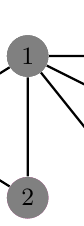
\begin{tikzpicture}[scale=1.8,auto,swap]
            \onslide<1>{
                \node[vertex] (0) at (0,0.5) {0};
                \node[vertex] (1) at (0.8,1) {1};
                \node[vertex] (2) at (0.8,0) {2};
                \node[vertex] (3) at (2,1) {3};
                \node[vertex] (4) at (1.8,0.5) {4};
                \node[vertex] (5) at (1.6,0) {5};
            }
            \onslide<2-3>{
                \node[vertex] (0) at (0,0.5) {0};
                \node[vertex] (1) at (0.8,1) {1};
                \node[selected vertex] (2) at (0.8,0) {2};
                \node[selected vertex] (3) at (2,1) {3};
                \node[vertex] (4) at (1.8,0.5) {4};
                \node[selected vertex] (5) at (1.6,0) {5};
            }
            \onslide<4->{
                \node[selected vertex] (0) at (0,0.5) {0};
                \node[vertex] (1) at (0.8,1) {1};
                \node[vertex] (2) at (0.8,0) {2};
                \node[selected vertex] (3) at (2,1) {3};
                \node[selected vertex] (4) at (1.8,0.5) {4};
                \node[selected vertex] (5) at (1.6,0) {5};
            }

            \path[edge] (0) -- (1);
            \path[edge] (0) -- (2);
            \path[edge] (1) -- (2);
            \path[edge] (1) -- (3);
            \path[edge] (1) -- (4);
            \path[edge] (1) -- (5);

            \pgfresetboundingbox
            \path [use as bounding box] (0.8,0) rectangle (1,1.2);
        \end{tikzpicture}
    \end{figure}

    \vspace{10pt}
    \bi
        \item<3-> We want to find an independent set of maximum size
        \vspace{10pt}
        \item<5-> NP-hard problem in general graphs
    \ei
\end{frame}

\begin{frame}{Relation between MVC and MIS}
    \bi
        \item The previous two problems are very related
        \item A subset of the vertices is a vertex cover if and only if the complement of the set is an independent set
    \ei

    \begin{figure}
        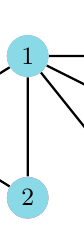
\begin{tikzpicture}[scale=1.8,auto,swap]
            \onslide<1>{
                \node[vertex] (0) at (0,0.5) {0};
                \node[vertex] (1) at (0.8,1) {1};
                \node[vertex] (2) at (0.8,0) {2};
                \node[vertex] (3) at (2,1) {3};
                \node[vertex] (4) at (1.8,0.5) {4};
                \node[vertex] (5) at (1.6,0) {5};
            }
            \onslide<2>{
                \node[selected2 vertex] (0) at (0,0.5) {0};
                \node[selected2 vertex] (1) at (0.8,1) {1};
                \node[selected vertex] (2) at (0.8,0) {2};
                \node[selected vertex] (3) at (2,1) {3};
                \node[selected2 vertex] (4) at (1.8,0.5) {4};
                \node[selected vertex] (5) at (1.6,0) {5};
            }
            \onslide<3->{
                \node[selected vertex] (0) at (0,0.5) {0};
                \node[selected2 vertex] (1) at (0.8,1) {1};
                \node[selected2 vertex] (2) at (0.8,0) {2};
                \node[selected vertex] (3) at (2,1) {3};
                \node[selected vertex] (4) at (1.8,0.5) {4};
                \node[selected vertex] (5) at (1.6,0) {5};
            }

            \path[edge] (0) -- (1);
            \path[edge] (0) -- (2);
            \path[edge] (1) -- (2);
            \path[edge] (1) -- (3);
            \path[edge] (1) -- (4);
            \path[edge] (1) -- (5);

            \pgfresetboundingbox
            \path [use as bounding box] (0.8,0) rectangle (1,1.2);
        \end{tikzpicture}
    \end{figure}

    \vspace{10pt}
    \bi
        \item<4-> The size of a minimum vertex cover plus the size of a maximum independent set is equal to the number of vertices
    \ei
\end{frame}

% TODO: Matching
\begin{frame}{Maximum matching}
    \bi
        \item We have an unweighted undirected graph
        \item A matching is a subset of the edges such that each vertex is adjacent to at most one edge in the subset
    \ei

    \begin{figure}
        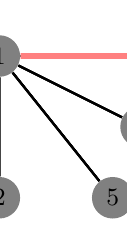
\begin{tikzpicture}[scale=1.8,auto,swap]
            \node[vertex] (0) at (0,0.5) {0};
            \node[vertex] (1) at (0.8,1) {1};
            \node[vertex] (2) at (0.8,0) {2};
            \node[vertex] (3) at (2,1) {3};
            \node[vertex] (4) at (1.8,0.5) {4};
            \node[vertex] (5) at (1.6,0) {5};
            \node[vertex] (6) at (2.4,0) {6};

            \onslide<1>{
                \path[edge] (0) -- (1);
                \path[edge] (0) -- (2);
                \path[edge] (1) -- (2);
                \path[edge] (1) -- (3);
                \path[edge] (1) -- (4);
                \path[edge] (1) -- (5);
                \path[edge] (5) -- (6);
            }
            \onslide<2-3>{
                \path[selected edge] (0) -- (1);
                \path[edge] (0) -- (2);
                \path[edge] (1) -- (2);
                \path[edge] (1) -- (3);
                \path[edge] (1) -- (4);
                \path[edge] (1) -- (5);
                \path[selected edge] (5) -- (6);
            }
            \onslide<4->{
                \path[edge] (0) -- (1);
                \path[selected edge] (0) -- (2);
                \path[edge] (1) -- (2);
                \path[selected edge] (1) -- (3);
                \path[edge] (1) -- (4);
                \path[edge] (1) -- (5);
                \path[selected edge] (5) -- (6);
            }

            \pgfresetboundingbox
            \path [use as bounding box] (1.5,0) rectangle (1,1.2);
        \end{tikzpicture}
    \end{figure}

    \vspace{10pt}
    \bi
        \item<3-> We want to find a matching of maximum size
        \vspace{10pt}
    \item<5-> There exists an $O(V^4)$ algorithm for general graphs, but is pretty complex (Hungarian algorithm)
    \ei
\end{frame}

% TODO: Coloring
\begin{frame}{Graph coloring}
    \bi
        \item We have an unweighted undirected graph
        \item A coloring of the graph is an assignment of colors to the vertices such that adjacent vertices have different colors
    \ei

    \begin{figure}
        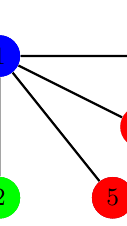
\begin{tikzpicture}[scale=1.8,auto,swap]
            \onslide<1>{
                \node[vertex] (0) at (0,0.5) {0};
                \node[vertex] (1) at (0.8,1) {1};
                \node[vertex] (2) at (0.8,0) {2};
                \node[vertex] (3) at (2,1) {3};
                \node[vertex] (4) at (1.8,0.5) {4};
                \node[vertex] (5) at (1.6,0) {5};
            }
            \onslide<2-3>{
                \node[vertex1] (0) at (0,0.5) {0};
                \node[vertex2] (1) at (0.8,1) {1};
                \node[vertex3] (2) at (0.8,0) {2};
                \node[vertex4] (3) at (2,1) {3};
                \node[vertex5] (4) at (1.8,0.5) {4};
                \node[vertex6] (5) at (1.6,0) {5};
            }
            \onslide<4->{
                \node[vertex1] (0) at (0,0.5) {0};
                \node[vertex2] (1) at (0.8,1) {1};
                \node[vertex3] (2) at (0.8,0) {2};
                \node[vertex1] (3) at (2,1) {3};
                \node[vertex1] (4) at (1.8,0.5) {4};
                \node[vertex1] (5) at (1.6,0) {5};
            }

            \path[edge] (0) -- (1);
            \path[edge] (0) -- (2);
            \path[edge] (1) -- (2);
            \path[edge] (1) -- (3);
            \path[edge] (1) -- (4);
            \path[edge] (1) -- (5);

            \pgfresetboundingbox
            \path [use as bounding box] (1.5,0) rectangle (1,1.2);
        \end{tikzpicture}
    \end{figure}

    \vspace{10pt}
    \bi
        \item<3-> We want to find a coloring that uses the minimum number of distinct colors
        \vspace{10pt}
        \item<5-> NP-hard in general graphs
    \ei

\end{frame}

\begin{frame}{Special graphs}
    \vspace{30pt}
    \bi
\item All of these problems are hard (in some sense) in general graphs
\item But what if we're working with special kinds of graphs?
    \vspace{10pt}
\item Let's look at a few examples
    \ei
\end{frame}

\begin{frame}{Bipartite graphs}
    \bi
\item A graph is bipartite if the vertices can be partitioned into two sets such that for each edge $(u,v)$ $u$ and $v$ are in different sets
% \item Bipartite graphs are the \textbf{$C_{2x+1}$-free} graphs
    \ei
    \begin{figure}
        \begin{tikzpicture}[scale=1.8,auto,swap]
            \only<-1>{
                \node[vertex] (0) at (0,0.5) {0};
            }
            \only<2->{
                \node[vertex] (0) at (0,0) {0};
            }
            \node[vertex] (1) at (0.8,1) {1};
            \node[vertex] (2) at (0.8,0) {2};
            \only<-3>{
                \node[vertex] (3) at (2,1) {3};
                \node[vertex] (4) at (1.8,0.5) {4};
                \node[vertex] (5) at (1.6,0) {5};
            }
            \only<4->{
                \node[vertex] (3) at (2,0) {3};
                \node[vertex] (4) at (1.6,0) {4};
                \node[vertex] (5) at (1.2,0) {5};
            }
            \only<-2>{
                \node[vertex] (6) at (0,-0.5) {6};
            }
            \only<3->{
                \node[vertex] (6) at (0,1) {6};
            }

            \path[edge] (0) -- (1);
            \path[edge] (0) -- (6);
            \path[edge] (6) -- (2);
            \path[edge] (1) -- (2);
            \path[edge] (1) -- (3);
            \path[edge] (1) -- (4);
            \path[edge] (1) -- (5);

            \onslide<5->{
                \draw[color=vhilight] (0.4,1) ellipse (0.7cm and 0.3cm);
                \draw[color=vhilight] (1.0,0) ellipse (1.5cm and 0.3cm);
            }

            \pgfresetboundingbox
            \path [use as bounding box] (1.5,0) rectangle (1,1.2);
        \end{tikzpicture}
    \end{figure}

    \vspace{20pt}
    \bi
        \item How do we check if a graph is bipartite?
    \ei
\end{frame}

\begin{frame}{Bipartite graphs}
    \vspace{10pt}
    \bi
        \item We want to check if we can split the vertices into these two groups
        \item Take any vertex, and assume that it's in the first group
        \item Then all of his neighbors must be in the second group
        \item And then all of their neighbors must be in the first group
        \item And so on...
        \vspace{10pt}
        \item We can do this with a simple depth-first search
        \item If we ever find a contradiction (i.e.\ a vertex must both be in the first and second set), then the graph is not bipartite
    \ei
\end{frame}

\begin{frame}[fragile]{Bipartite graphs}
    \begin{minted}[fontsize=\scriptsize]{cpp}
vi adj[1000];
int side[1000];
bool is_bipartite = true;

void check_bipartite(int u) {
    FORIT(i,adj[u])
        if (side[*i] == -1) {
            side[*i] = 1 - side[u];
            check_bipartite(*i);
        } else if (side[u] == side[*i]) {
            is_bipartite = false;
        }
}

FOR(i,0,1000) side[i] = -1
FOR(i,0,1000) if (side[u] == -1) {
    side[i] = 0;
    check_bipartite(i);
}
    \end{minted}
\end{frame}

\begin{frame}{Cliques in bipartite graphs}
    \bi
        \item ... well all maximum cliques have size 2
    \ei
\end{frame}

\begin{frame}{Coloring bipartite graphs}
    \bi
        \item What if we want to find the minimum graph coloring of a bipartite graph?
    \ei

    \begin{figure}
        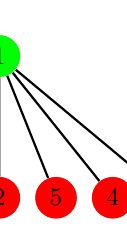
\begin{tikzpicture}[scale=1.8,auto,swap]
            \onslide<-1>{
                \node[vertex] (0) at (0,0) {0};
                \node[vertex] (1) at (0.8,1) {1};
                \node[vertex] (2) at (0.8,0) {2};
                \node[vertex] (3) at (2,0) {3};
                \node[vertex] (4) at (1.6,0) {4};
                \node[vertex] (5) at (1.2,0) {5};
                \node[vertex] (6) at (0,1) {6};
            }
            \onslide<2->{
                \node[vertex1] (0) at (0,0) {0};
                \node[vertex3] (1) at (0.8,1) {1};
                \node[vertex1] (2) at (0.8,0) {2};
                \node[vertex1] (3) at (2,0) {3};
                \node[vertex1] (4) at (1.6,0) {4};
                \node[vertex1] (5) at (1.2,0) {5};
                \node[vertex3] (6) at (0,1) {6};
            }

            \path[edge] (0) -- (1);
            \path[edge] (0) -- (6);
            \path[edge] (6) -- (2);
            \path[edge] (1) -- (2);
            \path[edge] (1) -- (3);
            \path[edge] (1) -- (4);
            \path[edge] (1) -- (5);

            \pgfresetboundingbox
            \path [use as bounding box] (1.5,0) rectangle (1,1.2);
        \end{tikzpicture}
    \end{figure}

    \vspace{20pt}
    \bi
        \item<2-> Simple, one side can be colored with one color, and the second side can be colored with a second color
    \ei
\end{frame}

\begin{frame}{Bipartite matching}
    \vspace{30pt}
    \bi
        \item Finding a maximum matching in bipartite graphs is very common
      %  \item \textit{see example}
      %      \vspace{10pt}
        \item Next time we'll see an efficient algorithm for finding the maximum matching in a bipartite graph
        \item Remember that an efficient algorithm (runtime $\leq O(n^3)$) for finding maximum matchings in large general graphs is not known
    \ei
\end{frame}

\begin{frame}{König's theorem}
    \vspace{10pt}
    \bi
        \item König's theorem states that the size of a minimum vertex cover in a bipartite graph is equal to the size of the maximum matching in that graph
        \vspace{10pt}
        \item So to find the minimum vertex cover in a bipartite graph, we just find the maximum matching with our efficient algorithm, and we have our answer
        \item And since the size of the maximum independent set is just the number of vertices minus the size of the minimum vertex cover, we can also compute the maximum independent set for a bipartite graph efficiently
    \ei
\end{frame}

\begin{frame}{Trees}
    \vspace{20pt}
    \bi
\item An undirected graph is a tree if it has no cycles
    \vspace{10pt}
\item Easy to check if a graph is a tree by checking if there are any backward edges in the depth-first search tree (see previous lecture)
\vspace{10pt}
\item A connected tree with $n$ vertices has exactly $n-1$ edges
\vspace{10pt}
\item Between each pair of vertices $u,v$ in the tree, there exists exactly one simple path, which can be found with depth-first search (or breadth-first search)
    \ei
\end{frame}

\begin{frame}{Trees}
    \vspace{10pt}
    \bi
\item What if we look at these problems for trees?
    \vspace{10pt}
\item How do we find the minimum number of colors needed to color a tree?

    \onslide<2->{
        \vspace{10pt}
        \item Well, trees are actually bipartite graphs...
        \item Why? Pick some vertex and make it the root of the tree. Then vertices at even heights in the tree can be put on one side, and vertices at odd heights can be put on the other side
        \vspace{10pt}
        \item So all the efficient algorithms for bipartite graphs also work for trees
    }
    \ei
\end{frame}

\begin{frame}{Trees}
    \vspace{30pt}
    \bi
        \item Trees are also well suited for dynamic programming, so many problems become simpler here because of that
        \item Base case: a leaf (only one connected edge)
        \item Recursive case: inner nodes (more then one connected edge)
    \ei
\end{frame}

\begin{frame}{Directed acyclic graphs}
    \vspace{20pt}
    \bi
        \item A directed graph is a directed acyclic graph if it doesn't contain any cycles
    \vspace{10pt}
\item Easy to check if a graph is a DAG by checking if there are any backward edges in the depth-first search tree (see previous lecture)
    \vspace{10pt}
\item Many problems are simple on DAGs, since it's easy to do dynamic programming over DAGs
        \bi
            \item counting number of simple paths from $u$ to $v$
            \item longest simple path from $u$ to $v$
        \ei
    \ei
\end{frame}


\begin{frame}{Cordal graphs}
     \bi
 \item Cordal graphs are the \textbf{induced $C_i$-free} ($i \geq 4$) graphs
     \ei
  \begin{figure}
    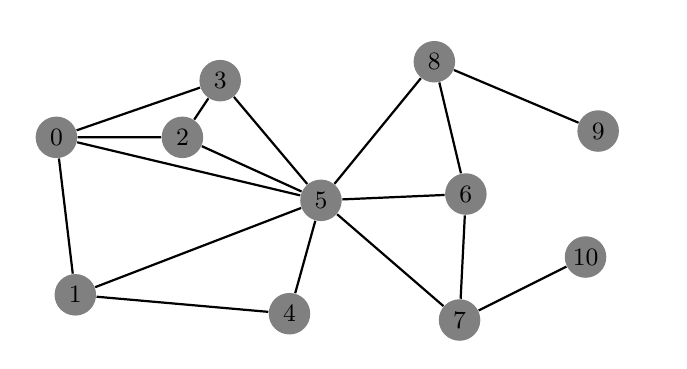
\begin{tikzpicture}[auto, swap,scale=0.8]
			\node at (-0.5,3.5) {\phantom{a}};
			\node at (9,3.5) {\phantom{a}};
      \node<1->[vertex] (0) at (-0.3,2) {0};
      \node<1->[vertex] (1) at (0.0,-0.5) {1};
      \node<1->[vertex] (2) at (1.7,2.0) {2};
      \node<1->[vertex] (3) at (2.3,2.9) {3};
      \node<1->[vertex] (4) at (3.4,-0.8) {4};
	  \node<1->[vertex] (5) at (3.9,1) {5};
     
	  \node<1->[vertex] (6) at (6.2,1.1) {6};
      \node<1->[vertex] (7) at (6.1,-0.9) {7};
	  \node<1->[vertex] (8) at (5.7,3.2) {8};
			
	  \node<1->[vertex] (9) at (8.3,2.1) {9};
      \node<1->[vertex] (10) at (8.1,0.1) {10};

      \path[edge] (0) -- (2);
      \path<2->[edge] (0) -- (5);

      \path[edge] (1) -- (0);
      \path[edge] (1) -- (4);

      \path[edge] (2) -- (3);

      \path[edge] (3) -- (0);

      \path[edge] (4) -- (5);

      \path[edge] (5) -- (1);
      \path[edge] (5) -- (2);
      \path[edge] (5) -- (3);
      \path[edge] (5) -- (6);
      \path[edge] (5) -- (7);
      \path[edge] (5) -- (8);

      %\path[dedge] (6) -- (5);
      \path[edge] (6) -- (8);
      \path[edge] (6) -- (7);

      %\path[dedge] (8) -- (5);
      \path[edge] (8) to (9);


      \path[edge] (7) -- (10);

       \end{tikzpicture}
  \end{figure}
\bi
	\item Chordal graphs have \emph{perfect elimination orders} $\langle v_1, \dots v_n \rangle$
	\item In a peo for every $v_i$: the neighbours $v_j$ of $v_i$ with $j > i$ form a clique
	\item Maximum Clique? Colouring?
\ei
\end{frame}



%\begin{frame}{Split Graphs}
%		-- detection by induced subgraphs
%\end{frame}

%\begin{frame}{Steiner Tree}
%\end{frame}

%\begin{frame}{Leaf-Powers}
%\end{frame}

%\begin{frame}{Comparability Graphs}
%
%\end{frame}

%\begin{frame}{Courcelle's theorem}
%		Tree width and stuff
%\end{frame}


\end{document}

